\documentclass[11pt]{article}
\usepackage{amsmath,amssymb,amsthm}
\usepackage{graphicx}
\usepackage[margin=1in]{geometry}
\usepackage[table]{xcolor}
\usepackage{csvsimple}
\usepackage{enumitem}
\usepackage{float}
\usepackage{caption}
\usepackage{hyperref}

\captionsetup[table]{justification=raggedright,singlelinecheck=off,labelfont=bf}
\usepackage{subcaption}
\restylefloat{table}
\usepackage{fancyhdr}
\setlength{\parindent}{0pt}
\setlength{\parskip}{5pt plus 1pt}
\setlength{\headheight}{13.6pt}
\newcommand\question[2]{\vspace{.25in}\hrule\textbf{#1: #2}\vspace{.5em}\hrule\vspace{.10in}}
\renewcommand\part[1]{\vspace{.10in}\textbf{(#1)}}
\newcommand\algorithm{\vspace{.10in}\textbf{Algorithm: }}
\newcommand\correctness{\vspace{.10in}\textbf{Correctness: }}
\newcommand\runtime{\vspace{.10in}\textbf{Running time: }}
\pagestyle{fancyplain}
\lhead{\textbf{\NAME\ (\ANDREWID)}}
\rhead{Page \thepage}
\begin{document}


%Section A==============Change the values below to match your information==================
\newcommand\NAME{Turaga}  % your name
\newcommand\ANDREWID{nturaga1@jhmi.edu}     % your andrew id
%\newcommand\HWNUM{1}              % the homework number

\title{Differntial Methylation Analysis of H460 Parent and H460 Knock-in cell lines on 2.1M Nimblegen Array}
\author{Nitesh Turaga}
\maketitle



To compare the differential methylation regions of H460 Knock-in cell line and H460 parent cell line.The data was generated from Nimblegen 2.1M oligonucleotide microarrays. The raw Nimblegen data were {\tt .tif} images. There were a total of 6 samples, 3 for each cell line(H460 knock-in and H460 parent).Array images were processed with DEVA-v1.2 (Nimblegen software for automated feature extraction and data analysis). The TIF files were processed and converted to {\bf XYS} files for analysis. These files report the, {\bf X} - coordinate of the feature on the image, {\bf Y}-coordinate of the feature on the image, and the {\bf S}ignal - the flourescence intensity of the pixels that make the feature. The TIF files were also processed with DEVA using the DNA methylation work flow to identify peaks and generate a result for each sample.

%%%%%%%%%%%%%%%%%%%%%%%%%% 
\section*{Preliminary Assessments}
%%%%%%%%%%%%%%%%%%%%%%%%%%


General QC-analyses brought to light that the signal intensities and local enrichment at methylated sites were not large. The data quality was assessed by looking at the Enriched channel in the MeDIP array, where we expect every probe to have a signal. Since, the enriched channel has methylated DNA, a successful hybridization would indicate a signal. The array signal is calculated as the average percentile rank of the signal probes among the background probes. The score ranges between 0 to 100, where 100 indicates the ideal scenario or perfect hybridization. This quality score is calculated before any kind of normalization is done on the arrays.


\captionof{table}{Array quality scores}
\begin{table}[H]
    \begin{tabular}{|l|l|l|}
    \hline
    Sample ID                        & Status       & Quality Score     \\ \hline
    542586A01\_Slot9\_2012-07-24\_H460 & H460\_parent & 59.6  \\ \hline
    542737A01\_Slot13\_2012-07-24\_H460 & H460\_parent & 64.4  \\ \hline
    542857A01\_Slot18\_2012-07-24\_H460 & H460\_parent & 69.8  \\ \hline
	542671A01\_Slot6\_2012-07-24\_H460 & H460\_knockin & 71.2  \\ \hline
    542654A01\_Slot9\_2012-07-25\_H460 & H460\_knockin & 74.9  \\ \hline    
    542707A01\_Slot12\_2012-07-25\_H460 & H460\_knockin & 76.5   \\ \hline
    \end{tabular}

\end{table}

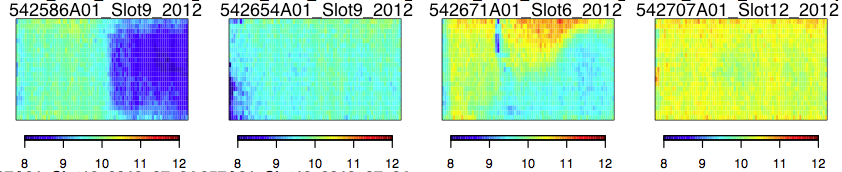
\includegraphics[scale=0.5]{qcImage1.png}

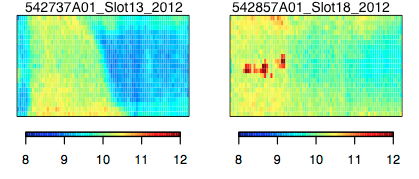
\includegraphics[scale=0.5]{qcImage2.png}


As we can in Table 1, the quality score of the H460 Parent arrays are pretty low.

%%%%%%%%%%%%%%%%%%%%%%%%%% 
\section*{The CHARM Algorithm}
%%%%%%%%%%%%%%%%%%%%%%%%%%

%Array quality scores were generated with the  Bioconductor {\tt charm - package}, and data quality was checked using the $Enriched$ channel. Four of the six arrays show a large standard deviation in the signal strenth and seem to have a problem in hybridization.
%
%To estimate the DNA methylation values, the background signal is removed before computing the log-ratios. A within sample normalization method - {\bf loess} is used, and then a between array normalization - quantile  is used. The control probes which are the non-CpG probes are excluded. This provides us a probe-level estimate of DNA methylation from the 2.1M oligonucliotide microarray.
%
%After estimating the DNA methylation values in terms of percentage methylation, we use the regression based DMR-finding approach after correcting for batch effects, which is provided by {\tt charm}. This fails to find DMR’s in the samples. Also, while not taking into account batch effects (surrogate variables), {\tt charm} does not find any DMR's. 

TODO: Needs to be edited (IN PROGRESS)


For each microarray hybridization, we used the raw feature intensities to form log ratios and denoted these with M. The M-values were formed so that larger values represented more evidence of methylation, e.g., with MeDIP, the immunoprecipitate intensity was in the numerator and the total DNA intensity in the denominator. Note that each feature on the array was associated with one M-value. Each array was then normalized so that unmethylated regions, on average, produced M-values of 0. We therefore developed a method that does not require the assumption that M = 0 for most probes. This method used genome sequence information and our knowledge of the fragment selection method to select what we call pseudo-housekeeping probes for which one can in fact assume M = 0. We then apply the Loess normalization procedure developed for expression arrays to the pseudo-housekeeping genes, obtain the correction curve, and use this curve to correct M-values for all probes.To obtain a smoothed M-value at any given genomic location, we average all the M-values that were within a prespecified distance from the location in question. The interval providing the values that are averaged is referred to as the “smoothing window” and its length is referred to as the “window size.”


%%%%%%%%%%%%%%%%%%%%%%%%%% 
\section*{The Bumphunter Algorithm}
%%%%%%%%%%%%%%%%%%%%%%%%%%


Bumphunter used to estimate regions for which the genomic profile deviates from a baseline value(cut off). It is implemented to detect differntially methylated genomic regions between two populations. It is also a regression based approach.It reports the result, with a table of candidate differentially methylated regions and the corresponding annotation for wach region.

%
%{\bf Analysis using Bumphunter}
%
%
%\begin{enumerate}
%
%\item Run  1
%
%Initially ran {\tt bumphunter} on the data, with cutoff value 1.0, this failed to find any bumps. The sensitivity of the cutoff was not enough to catch any DMRs in the sample set. Bumphunter is better used for large sample sets, for better performance. 
%
%
%\item Run  2
%
%Bumphunter, with the inbuilt argument to pickCutoff was run. The cutoff chosen by bumphunter was at 0.41, bumps found 28206. The number of DMRs/bumps of length greater than four is 0. This result is not useful for analysis as the length of the DMRs are too small.
%
%%bumps.rda file attached. 
%
%The distribution of the length of DMRs found, is shown below. Most of them are single CpG sites of length 1. This does not work for a significant analysis.
%
%\end{enumerate}
%
%\begin{table}[H]
%	\begin{tabular}{|l|l|l|l|}
%	\hline
%	Length(L) &   1     & 2   & 3 \\ \hline
%    Number of DMRs & 27981 & 222 & 3 \\ \hline
%	\end{tabular}
%	\caption{Distribution of Bumps}
%\end{table}
%
%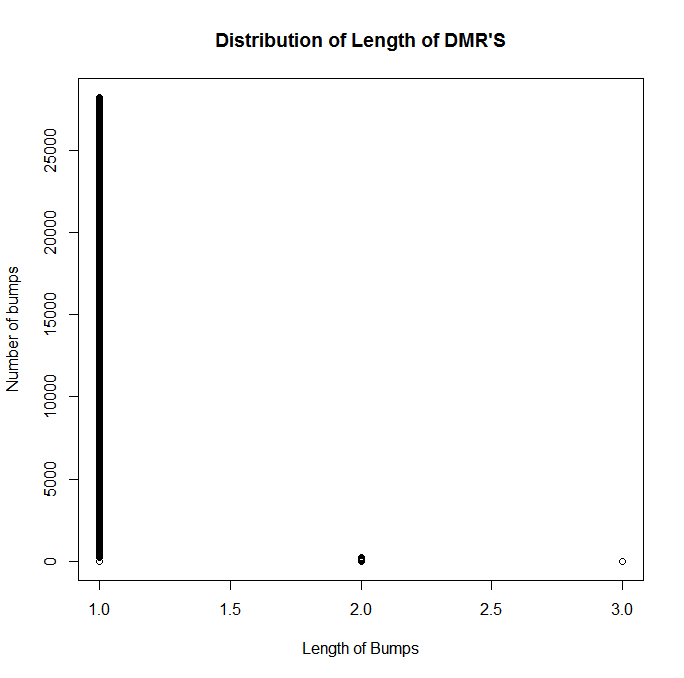
\includegraphics[scale=0.4]{bumpsDistribution.png}

%\begin{verbatim}
%Argument description for bumphunter,
%
%cutoff: 
%
%A numeric value. Values of the estimate of the genomic profile above the cutoff or
%below the negative of the cutoff will be used as candidate regions. It is possible to
%give two separate values (upper and lower bounds). If one value is given, the lower
%bound is minus the value.
%
%pickCutoff: 
%
%Should bumphunter attempt to pick a cutoff using the permutation
%distribution?
%
%\end{verbatim}


%%%%%%%%%%%%%%%%%%%%%%%%%% 
\section*{The Nimblegen Algorithm}
%%%%%%%%%%%%%%%%%%%%%%%%%%

The standard Nimblegen algorithms were used to compute the normalized data and identify peaks of enrichment, coinciding with methylated regions. Peaks near known transcription start sites (TSS) were identified, with different cutoffs between maximal distance between a peak and TSS.

%\begin{itemize}
%	\item  -500 to +500, the default cutoff
%	\item  -5000 to +1500, a custom cutoff
%\end{itemize}

%{\bf Analysis using Peaks files from DEVA}

In each cell line, the genes which were intersecting among all the samples were identified. All the genes which were identified jointly in both cell lines were removed, making each gene set unique and exclusive for a specific cell line. Both sets of unique and exclusive genes, were ordered by distance from the Transcription start site. 944 genes were identified in H460 knock-in cell line and 349 in H460 parent. (Table 2)

%Sequential intersections, based on the number of peaks identified in each sample, was done in decreasing order for each experimental status. This step results in all the genes within each sample which are intersecting.

%We find the common genes between “H460\_knock-in” and “H460\_parent", and remove these genes from the intersected lists. We then order them by distance from the transcription start site(TSS).

\captionof{table}{Number of features in each cell line}
\begin{table}[H]
\centering
	\begin{tabular}{|l|l|l|}
	\hline
		Cell line & Feature Track & Number of features \\ \hline
		H460 Knock in & transcription start site & 944 \\ \hline
		H460 Parent & transcription start site & 349 \\ \hline
	\end{tabular}
\end{table}

{\tt NOTE:  Files are attached as “knock-in\_genes\_distFromTSS.csv” and “parent\_genes\_distFromTSS.csv”. The regions are ordered in a decreasing order based on the distance from TSS.}


The only features left in the result are transcription start sites, other possible feature is CpG Island (column name  is  FEATURE TRACK). The distribution of the distance from the TSS is also shown for both cell lines. Column name is SHORTEST\_DISTANCE\_FROM\_FEATURE\_TO\_DATA\_POINT.

\captionof{table}{Summary of Feature distance from data point}
\begin{table}[H]
\centering
    \begin{tabular}{|l|l|l|l|l|l|l|}
    \hline
     Cell line & Min. & 1st Qu. & Median & Mean & 3rd Qu. &   Max.  \\ \hline
   H460 Knock in  & -4998.0 & -3363.0 & -1916.0 & -1956.0 & -569.8 & 995.0  \\ \hline
   H460 Parent & -4975 &  -3669 &  -2474 &  -2223 &   -718  &   997  \\ \hline
    \end{tabular}
\end{table}

\captionof{table}{Distribution of Shortest distance from feature to data point}
\begin{figure}[H]
\centering
\begin{subfigure}{.4\textwidth}
  %\centering
  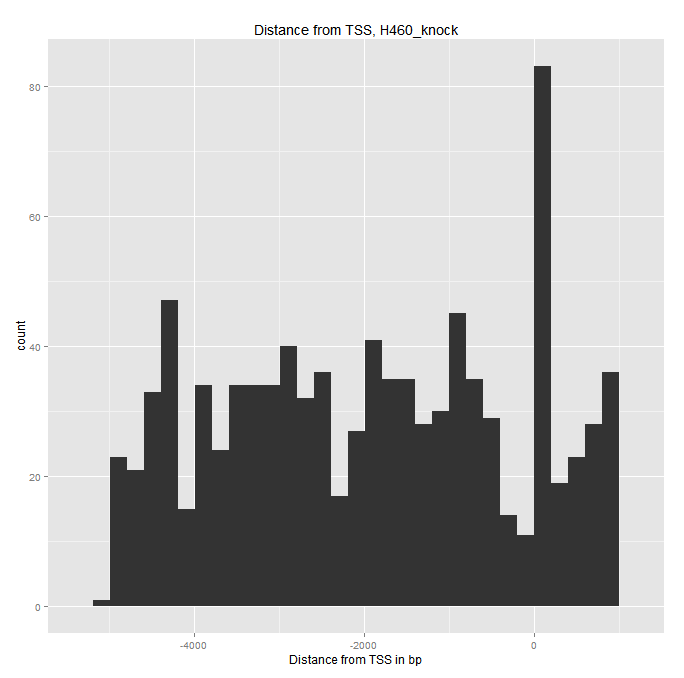
\includegraphics[scale=0.3]{distribution_knocking.png}
  \caption{H460 knock-in distance from TSS}
  \label{fig:sub1}
\end{subfigure}
\quad
\begin{subfigure}{.4\textwidth}
  %\centering
  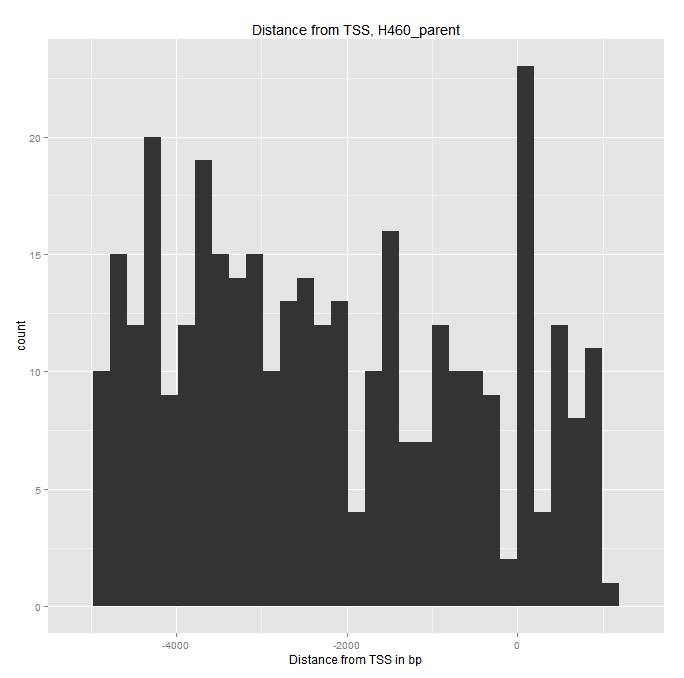
\includegraphics[scale=0.3]{distribution_parent.png}
  \caption{H460 parent distance from TSS}
  \label{fig:sub2}
\end{subfigure}

\label{fig:test}
\end{figure}



\newpage


%%%%%%%%%%%%%%%%%%%%%%%%%%
\section*{Pathway Comparisons}
%%%%%%%%%%%%%%%%%%%%%%%%%%

Both the list of H460 Knock-in genes and H460 parent genes were compared with a list of selected pathways.

\begin{enumerate}[itemsep=-0.2mm]
\item Cell Cycle                                 
\item Complete Homeobox (HOX) Genes                      
\item Complete Human Inflammatory Response and Autoimmunity 
\item Complete Human Tumor Suppressor Genes              
\item Complete Stem Cell Transcription Factors            
\item Complete Stress and Toxicity                         
\item Cytokine Production                                
\item DNA Repair 
\item Human Epithelial to Mesenchymal Transition (EMT)    
\item Human Notch Signaling Pathway                      
\item Human T-Cell B-Cell Activation Methylation         
\item Human T Helper Cell Differentiation                
\item Human Tumor Suppressor Genes                        
\item Inflammatory Response and Autoimmunity               
\item Polycomb and Trithorax Complexes                     
\item Stem Cell Transcription Factors                    
\item TGF f BMP Signaling Pathway                          
\item Toll-Like Receptor Signaling Pathway               
\item WNT Signaling Pathway                              
\end{enumerate}

Very few pathway genes matched with the H460 knock-in genes and the H460 parent genes. 

The H460 knock-in genes have only 29 genes in common with the pathways(listed in Table 5). The following result from shows you the pathways and the genes along with gene description. The result, for the names of the genes is stored in "pathway\_genes\_knock.csv". 

\newpage

\captionof{table}{H460 Knock-in gene with corresponding pathways}

\begin{table}[H]
	\resizebox{\columnwidth}{!}{%
    \begin{tabular}{|l|l|l|}
    \hline
    {\bf Gene name}   & {\bf Description}                                                                           & {\bf Pathway}                                  \\ \hline
    BRCA1  & breast cancer 1, early onset                                                          & Cell\_Cycle                              \\
    HOXB2  & homeobox B2                                                                           & Complete\_Homeobox\_(HOX)\_Genes         \\
    HOXB3  & homeobox B3                                                                           & Complete\_Homeobox\_(HOX)\_Genes         \\
    HOXB4  & homeobox B4                                                                           & Complete\_Homeobox\_(HOX)\_Genes         \\
    HOXB6  & homeobox B6                                                                           & Complete\_Homeobox\_(HOX)\_Genes         \\
    HOXB7  & homeobox B7                                                                           & Complete\_Homeobox\_(HOX)\_Genes         \\
    HOXB8  & homeobox B8                                                                           & Complete\_Homeobox\_(HOX)\_Genes         \\
    BRCA1  & breast cancer 1, early onset                                                          & Complete\_Human\_Tumor\_Suppressor\_Genes \\
    DIRAS3 & DIRAS family, GTP-binding RAS-like 3                                                  & Complete\_Human\_Tumor\_Suppressor\_Genes \\
    XRCC1  & X-ray repair complementing defective repair in Chinese hamster cells 1                & Complete\_Human\_Tumor\_Suppressor\_Genes \\
    GATA6  & GATA binding protein 6                                                                & Complete\_Stem\_Cell\_Transcription\_Factors \\
    HOXB3  & homeobox B3                                                                           & Complete\_Stem\_Cell\_Transcription\_Factors \\
    HOXB8  & homeobox B8                                                                           & Complete\_Stem\_Cell\_Transcription\_Factors \\
    SOX9   & SRY (sex determining region Y)-box 9                                                  & Complete\_Stem\_Cell\_Transcription\_Factors \\
    STAT3  & signal transducer and activator of transcription 3 (acute-phase response factor)      & Complete\_Stem\_Cell\_Transcription\_Factors \\
    ATF4   & activating transcription factor 4 (tax-responsive enhancer element B67)               & Complete\_Stress\_\&\_Toxicity           \\
    BRCA1  & breast cancer 1, early onset                                                          & Complete\_Stress\_\&\_Toxicity           \\
    ERCC1  & excision repair cross-complementing rodent repair deficiency, complementation group 1 & Complete\_Stress\_\&\_Toxicity           \\
    GPX7   & glutathione peroxidase 7                                                              & Complete\_Stress\_\&\_Toxicity           \\
    SMC1A  & structural maintenance ofchromosomes 1A                                               & Complete\_Stress\_\&\_Toxicity           \\
    XRCC1  & X-ray repair complementing defective repair in Chinese hamster cells 1                & Complete\_Stress\_\&\_Toxicity           \\
    ELANE  & elastase, neutrophil expressed                                                        & Cytokine\_Production                     \\
    BRCA1  & breast cancer 1, early onset                                                          & DNA\_Repair                              \\
    XRCC1  & X-ray repair complementing defective repair in Chinese hamster cells 1                & DNA\_Repair                              \\
    PSENEN & presenilin enhancer 2 homolog (C. elegans)                                            & Human\_Notch\_Signaling\_Pathway         \\
    BRCA1  & breast cancer 1, early onset                                                          & Human\_Tumor\_Suppressor\_Genes          \\
    CBX2   & chromobox homolog 2 (Pc class homolog, Drosophila)                                    & Polycomb\_\&\_Trithorax\_Complexes       \\
    STAT3  & signal transducer and activator of transcription 3 (acute-phase response factor)      & Stem\_Cell\_Transcription\_Factors       \\
    IRAK1  & interleukin-1 receptor-associated kinase 1                                            & Toll-Like\_Receptor\_Signaling\_Pathway  \\ \hline
    \end{tabular}}
\end{table}


The H460 parent genes have only 2 genes in two pathways(Table 6) , and stored in "pathways\_genes\_parent.csv".

\captionof{table}{H460 parent gene with corresponding pathways }
\begin{table}[H]
    \begin{tabular}{|l|l|l|}
    \hline
    {\bf Gene name} & {\bf Description}       & {\bf Pathway}                                  \\ \hline
    AR   & androgen receptor & Complete\_Stem\_Cell\_Transcription\_Factors \\ 
    AR   & androgen receptor & Stem\_Cell\_Transcription\_Factors       \\ \hline
    \end{tabular}
\end{table}



DEVA was also run with a changed cutoff of -5000 to +1500 to produce peak files. A similar pipeline was run as with the new peak files as described above for pathway analysis. The results were different as expected because of a bigger window size. 

\captionof{table}{Number of features in each cell line with extended window}
\begin{table}[H]
\centering
	\begin{tabular}{|l|l|l|}
	\hline
		Cell line & Feature Track & Number of features \\ \hline
		H460 Knock in & transcription start site & 3877 \\ \hline
		H460 Parent & transcription start site & 2639 \\ \hline
	\end{tabular}
\end{table}

The pathway analysis showed, in the H460 Knock-in gene set 189 genes were observed in 18 pathways and in the H460 parent gene set 70 genes were observed in 19 pathways. 
%Please click on references 5 and 6 for H460 knock-in and H460 parent respectively.




%%%%%%%%%%%%%%%%%%%%%%%%%%
\section*{R-packages Used}
%%%%%%%%%%%%%%%%%%%%%%%%%%

List of R-packages used for analysis:
\begin{enumerate}

\item Charm

\item Bioconductor

\item BiocGenerics

\item plyr

\item RCircos

\end{enumerate}




%%%%%%%%%%%%%%%%%%%%%%%%%%
\section*{References}  
%%%%%%%%%%%%%%%%%%%%%%%%%%
\begin{enumerate}


	\item  Aryee MJ et al., Accurate genome-scale percentage DNA methylation estimates
	  from microarray data, Biostatistics (2011) 12(2): 197-210 	

	\item  Seth Falcon, Benilton Carvalho with contributions by Vince Carey, Matt
	  Settles and Kristof de Beuf. pdInfoBuilder: Platform Design Information
	  Package Builder. R package version 1.24.0.
	
	\item   Rafael A. Irizarry, Martin Aryee, Hector Corrada Bravo, Kasper D. Hansen and	Harris A. Jaffee (). bumphunter: Bump Hunter. R package version 1.0.0.
		
	\item RCircos: an R package for Circos 2D track plots
	
%	\item \href{https://app.box.com/s/7xr01qkv3xx41oo5izew}{H460 knock-in genes with corresponding pathways(Click here)} 
%	
%	\item \href{https://app.box.com/s/pu0n89gusqlf1umjwwhh}{H460 parent genes with corresponding pathways(Click here)}

	\item Irizarry RA, Ladd-Acosta C, Carvalho B, et al. Comprehensive high-throughput arrays for relative methylation (CHARM) Genome Res. 2008;18(5):780–790. 
\end{enumerate}

 
 
 
 
 \end{document}


